\section{The modular tessellation and the exponential transformation}

In the theory of modular functions, which we will touch in the next section,
a map of essential importance is the transformation $z \mapsto \exp(2 \pi \ii z)$, as it prominently occurs in Fourier expansions of modular functions -- compare for example \Petersson{} and \Rademacher{}. Adopting the notation of \Lehner{}, we will denote this transformation by
\begin{equation}
\label{eqn_ExponentialTransform}
\ex(z) := \exp\left(2 \pi \ii z \right).
%\fundef{\ex}{\C}{\C}{z}{\exp\left(2 \pi \ii z\right)}.
\end{equation}
Just like the Cayley transform, $\ex$ maps the upper half-plane onto the unit disk $\mathbb{D}$, as we see through
\begin{equation*}
\abs{\ex(z)} = 
\exp\left(\Re{2 \pi \ii z}\right) = 
\exp\left(-2 \pi \Im{z}\right).
\end{equation*}
Obviously $\Im{z} > 0$ implies $\abs{\ex(z)} < 1$. The real axis is mapped to the boundary of $\mathbb{D}$. In contrast to the Cayley transform, $e$ is not a one-to-one map from the upper half-plane to the unit disk, as clearly $e(z) = e(z + k)$ for arbitrary $k \in \Z$. Instead it can be considered as a bijective map from the strip 
\begin{equation*}
S = \setdefsz{\big}{z \in \C}{\Re{z} \in \left[-0.5,0.5\right),\ \Im{z} \ge 0}
\end{equation*}
to the punctured unit disk $\mathbb{D} \setminus \{0\}$. Note that the exponential function has an essential singularity at the point $\infty$, but still it is sometimes useful to define $e(\infty) := 0$. This is motivated by a continuous extension of $e$ from the domain $S$ to $S_\infty := S \cup \{\infty\}$ by
\begin{equation*}
e(\infty) := \lim_{\substack{\Im{z} \to \infty\\z \in S}} e(z) = 0.
\end{equation*}
In this way we obtain a bijective map from the set $S_\infty$ to the closed unit disk $\mathbb{D}$. Figure~\ref{fig_ModularTilingExp} shows the modular tessellation of the upper half-plane -- to be precise the part of it lying within $S_\infty$ -- mapped to the unit disk by $z \mapsto e(z).$
\begin{figure}
\centering
\includegraphics[width=\textwidth]{figures/modular-tiling-exp}
\caption[The modular tessellation under $z \mapsto \exp(2 \pi \ii z)$]{The modular tessellation under the transformation $z \mapsto e(z)$. The equation $\abs{z} = \exp(-2\pi \ii \Im{z})$ implies that points with large imaginary part are mapped very closely to $0$. For this reason, the image of the fundamental domain $\FunDom$ cannot be seen any more in this scale. Its points, satisfying $\Im{z} > \frac{\sqrt{3}}{2}$, are mapped into a disk centered about the origin of a radius smaller than $0.005$.}
\label{fig_ModularTilingExp}
\end{figure}

\begin{remark}
In order to trace the image of the fundamental domain $\FunDom$ and its indisk $\Indisk$ under the map $\ex$, we have to zoom in on the neighborhood of zero, which is done in Figure~\ref{fig_ModularTilingExpZoom}. The top-left frame again shows the image of the tessellation under $\ex$ on the whole unit disk. 

The second frame displays the images of the regions $TU\FunDom$ and $T\inv{U}\FunDom$ in more detail. Comparing with Figure~\ref{fig_ModularTiling}, we see that originally these two regions do not have any boundary arc in common. However, due to the periodicity of $e$, the left boundary arc of $TU\FunDom$ (being a segment of the line $\Re{z} = -1/2$) and the right boundary arc of $T\inv{U}\FunDom$ (being a segment of the line $\Re{z} = 1/2$) have the same image under the transformation $\ex$. Therefore the images of $TU\FunDom$ and $T\inv{U}\FunDom$ touch each other along a certain interval on the negative real axis. 

The third frame reveals some more detail on the real shape of $e(T\FunDom)$. Its ``tip'' is not round, as a short look on the first two frames might suggest, but in fact it has a kink at the point $\ex(\rho) = \ex(T\rho) \approx -0.0043$. Moreover, the image of $T\FunDom$ completely surrounds the image of the fundamental domain $\FunDom$ as we see in the next frame: 

Denoting the boundary arcs of $\FunDom$ by $a,b,c$ and $d$ as in Figure~\ref{fig_PSL2FunDom}, we can see in the fourth frame the image of the left boundary arc $a$ and the right boundary arc $b$ of $\FunDom$ are both mapped to the same interval $[\ex(\rho), 0]$ on the negative real axis. The images of the unit circle arcs $c$ and $d$ form the drop-shaped boundary of $\ex(\FunDom)$. Note that $\ex(c)$ constitutes the part of the boundary in the lower half-plane and $\ex(d)$ the part in the upper half-plane. 

Finally in the last row, we can see the image of the indisk $\Indisk$ in detail. Note that the transformed indisk touches itself in the point $\ex(\pm\half{1} + \half{3}\ii) \approx -0.00008$. The points within $\FunDom$ lying ``above'' $\Indisk$ (including the point $\infty$) are mapped to just another tiny drop-shaped region surrounded entirely by $\ex(\Indisk)$.

\begin{figure}
\centering
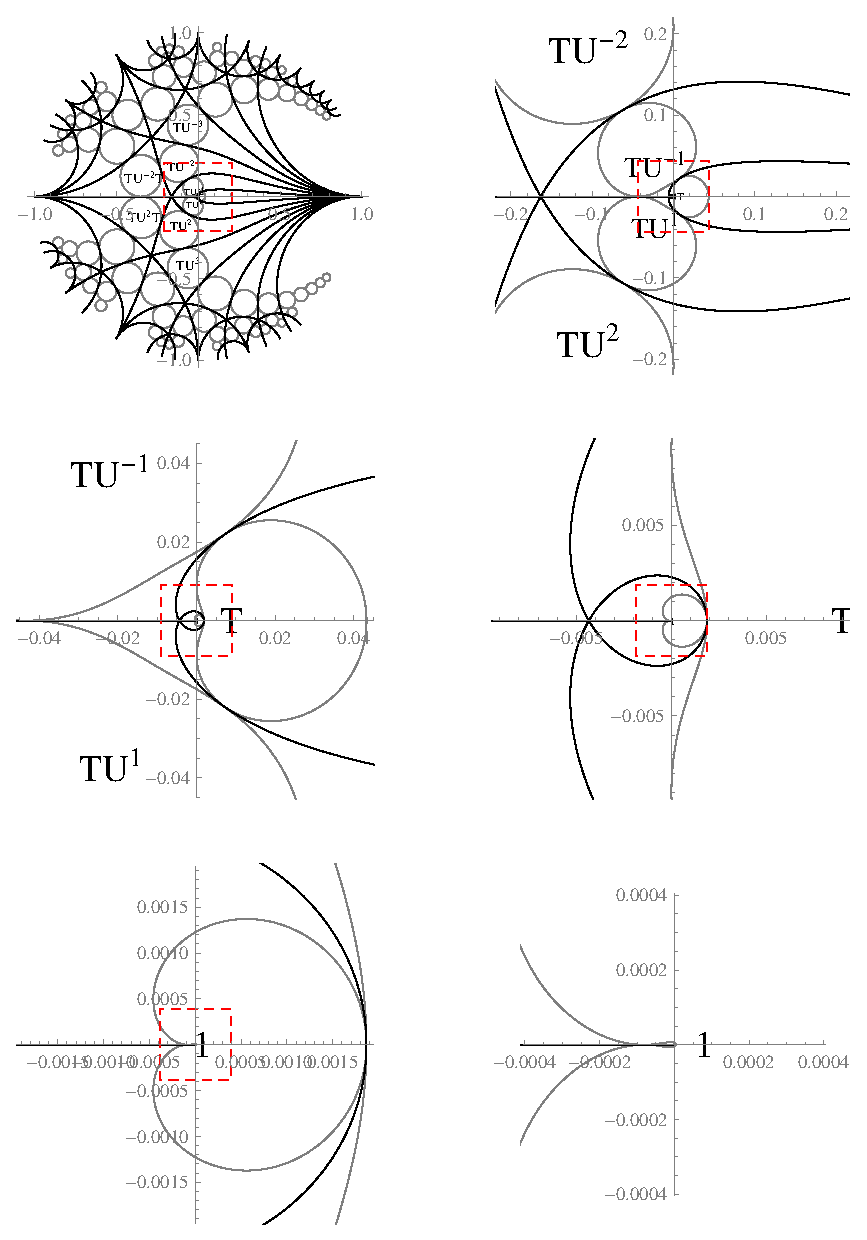
\includegraphics[width=0.95\textwidth]{figures/modular-tiling-exp-zoom}
\caption[The fundamental domain under $z \mapsto \exp(2 \pi \ii z)$]{The image of the fundamental domain $\FunDom$ and its indisk $\Indisk$ under the map $z \mapsto \ex(z)$ can be seen by zooming in to a close neighborhood of $0$.}
\label{fig_ModularTilingExpZoom}
\end{figure}
\end{remark}

Having studied the image of the modular tessellation under the transformation $z \mapsto \ex(z)$ in detail, the question arises whether this relates somehow to the image of the tessellation under the modified Cayley transform $\ModCayley$ which we have seen in Figure~\ref{fig_ModularTiling}. Indeed it is possible to visualize the connection between these two images. For this purpose we take advantage of yet another M�bius transformation:
\begin{equation}
f(z) := \frac{\ii}{z + \\i} = -\half{\ii} \ModCayley(z) + \half{1}.
\end{equation}
As we see, $f$ can be considered as composition of the modified Cayley transform, a clockwise rotation by $90^\circ$, scaling by the factor $\reci{2}$ and a final translation by $\reci{2}$. Therefore, $f$ maps the upper half-plane to a disk of radius $\reci{2}$ centered about the real point $\reci{2}$. The choice of $f$ is not as arbitrary as it first might seem, because
\begin{equation*}
f(0) = \ex(0) = 1 \quad\text{and}\quad f(\infty) = \ex(\infty) = 0.
\end{equation*}
This property allows it to establish a continuous transition between the images of the tessellation under $f$ and $\ex$ which leaves the points $0$ and $1$ fixed. For this purpose we may for example use the map
\begin{equation}
h(t, z) := f(z)^{1-t} \cdot \ex(tz),
\end{equation}
with varying parameter $t \in [0,1]$. Note that complex powers $z^t$, $z \in \C$, $t \in \R$ shall be evaluated as $\exp(t \ln z)$, by choosing a branch of the natural logarithm such that the imaginary part of the logarithm ranges in the interval $(-\pi, \pi]$. Moreover, for $z = \infty$ we define $h(t, \infty) := f(\infty) = \ex(\infty) = 0$.

In Figure~\ref{fig_ModularTilingExpFan}, we can see the images the modular tessellation under the map $h(t,\cdot)$ for the parameter values $t \in \{0,\reci{5},\frac{2}{5},\frac{3}{5},\frac{4}{5},1\}$. In the first frame, we see that the image of the tessellation under $h(0,\cdot) = f$ is indeed a rotated and scaled version of the one belonging to $\ModCayley$, when omitting the part which lies outside the strip $\abs{\Re{z}} \le \reci{2}$ (compare with Figure~\ref{fig_ModularTiling}). 

As the parameter value $t$ is stepwise increased in the following frames, the image is slowly fanned out to the whole unit disk. Finally we end up with the image of the tessellation under $h(1,\cdot) = \ex$.
\begin{figure}
\centering
\includegraphics[width=0.9\textwidth]{figures/modular-tiling-exp-fan}
\caption[The modular Pac-Man]{The modular tessellation on the strip $\abs{\Re{z}} \le \reci{2}$ under the maps $z \mapsto f(z) = \frac{\ii}{z + \\i}$ (top-left) and under $z \mapsto \ex(z)$ (bottom-right). A continuous transition between these two images is established through the map $h(t,z) = f(z)^{1-t} \cdot \ex(tz)$ when the parameter $t \in [0,1]$ is varied.}
\label{fig_ModularTilingExpFan}
\end{figure}

\begin{remark}
In a more general context, the connection between a region $R$ of similar shape as above (\ie a region bounded by three circular arcs having vertex angles $90^\circ$, $90^\circ$ and $0^\circ$), a parabolic M�bius transformation leaving the vertex with angle $0^\circ$ fixed and an exponential transformation which maps $R$ to the unit disk, is discussed in \Lehner{}, p.\ 68ff.
\end{remark}
\clearpage
